% Teilauswertung X

\section{Empfindlichkeit der FM-Apparatur und Konversionsverluste des Mischers}
\label{sec:verlusteAuswertung}

\subsection{Vergleich der Spektrumanalysatorwerte}
\label{sub:specAnalVergleich}

Zuerst wird die Theorie mit der Praxis verglichen. Dafür werden die gemessenen Werte des Spektrumanalysators aus Kapitel \ref{sub:verluste} [Tab. \ref{tab:specAnal}] zu den theoretischen Werten mit $P^*_\mathrm{S,Theo} = -30$\,dBm und für $P^*_\mathrm{R,Theo}= -79$\,dBm aus Kapitel \ref{sec:rauschen} \& \ref{sec:signalAbsorp} in Kontrast gesetzt. In Abbildung \ref{fig:specAnalVergleich} lässt sich erkennen, dass für die gemessenen Modulationsfrequenz $\omega_\mathrm{m}$ alle Leistungswerte im Bereich der Erwartung, in der Nähe der theoretischen Werte, liegen. Nur Werte für Modulationsfrequenzen von 400 $\sim$ 1350\,MHz weichen von der Theorie ab, was aber mit einem systematischen Messfehler zusammenhängen kann. Der Mittelwert der gemessenen Werte ist dabei:
\begin{gather}
    \boxed{\bar{P}^*_\mathrm{S,Mess} = (-23 \pm 1)\,\mathrm{dBm}} \qquad \boxed{\bar{P}^*_\mathrm{R,Mess} = (-78 \pm 1)\,\mathrm{dBm}}~.
\end{gather}

\subsection{Konversionsverluste}
\label{sub:konversionsverluste}

Nun werden die Werte des Spektrumanalysators, welcher die Werte nach HF-Verstärker am R-Eingang des Mischer gemessen hat, mit den Werten nach dem NF-Verstärkers verglichen. Dafür werden die Werte in Tabelle \ref{tab:verluste} durch den Faktor 31,5 geteilt \cite{anleitung}, um die Spannung $U_\mathrm{I}$ vor den NF-Verstärkers zu erhalten. Danach wird angenommen, dass der Mischer ohne Konversionsverluste arbeitet, d.h. Eingang L und R haben keine Phasendifferenz, womit die Spannung am Ausgang I gleich der Spannung am Ausgang R ist, also $U_\mathrm{R} = U_\mathrm{I}$. Eine skizzenhafte Darstellung des Schaltplans zur Übersicht ist in Abbildung \ref{fig:schaltschema} gegeben.

\begin{center}
    \captionsetup{type=figure}
    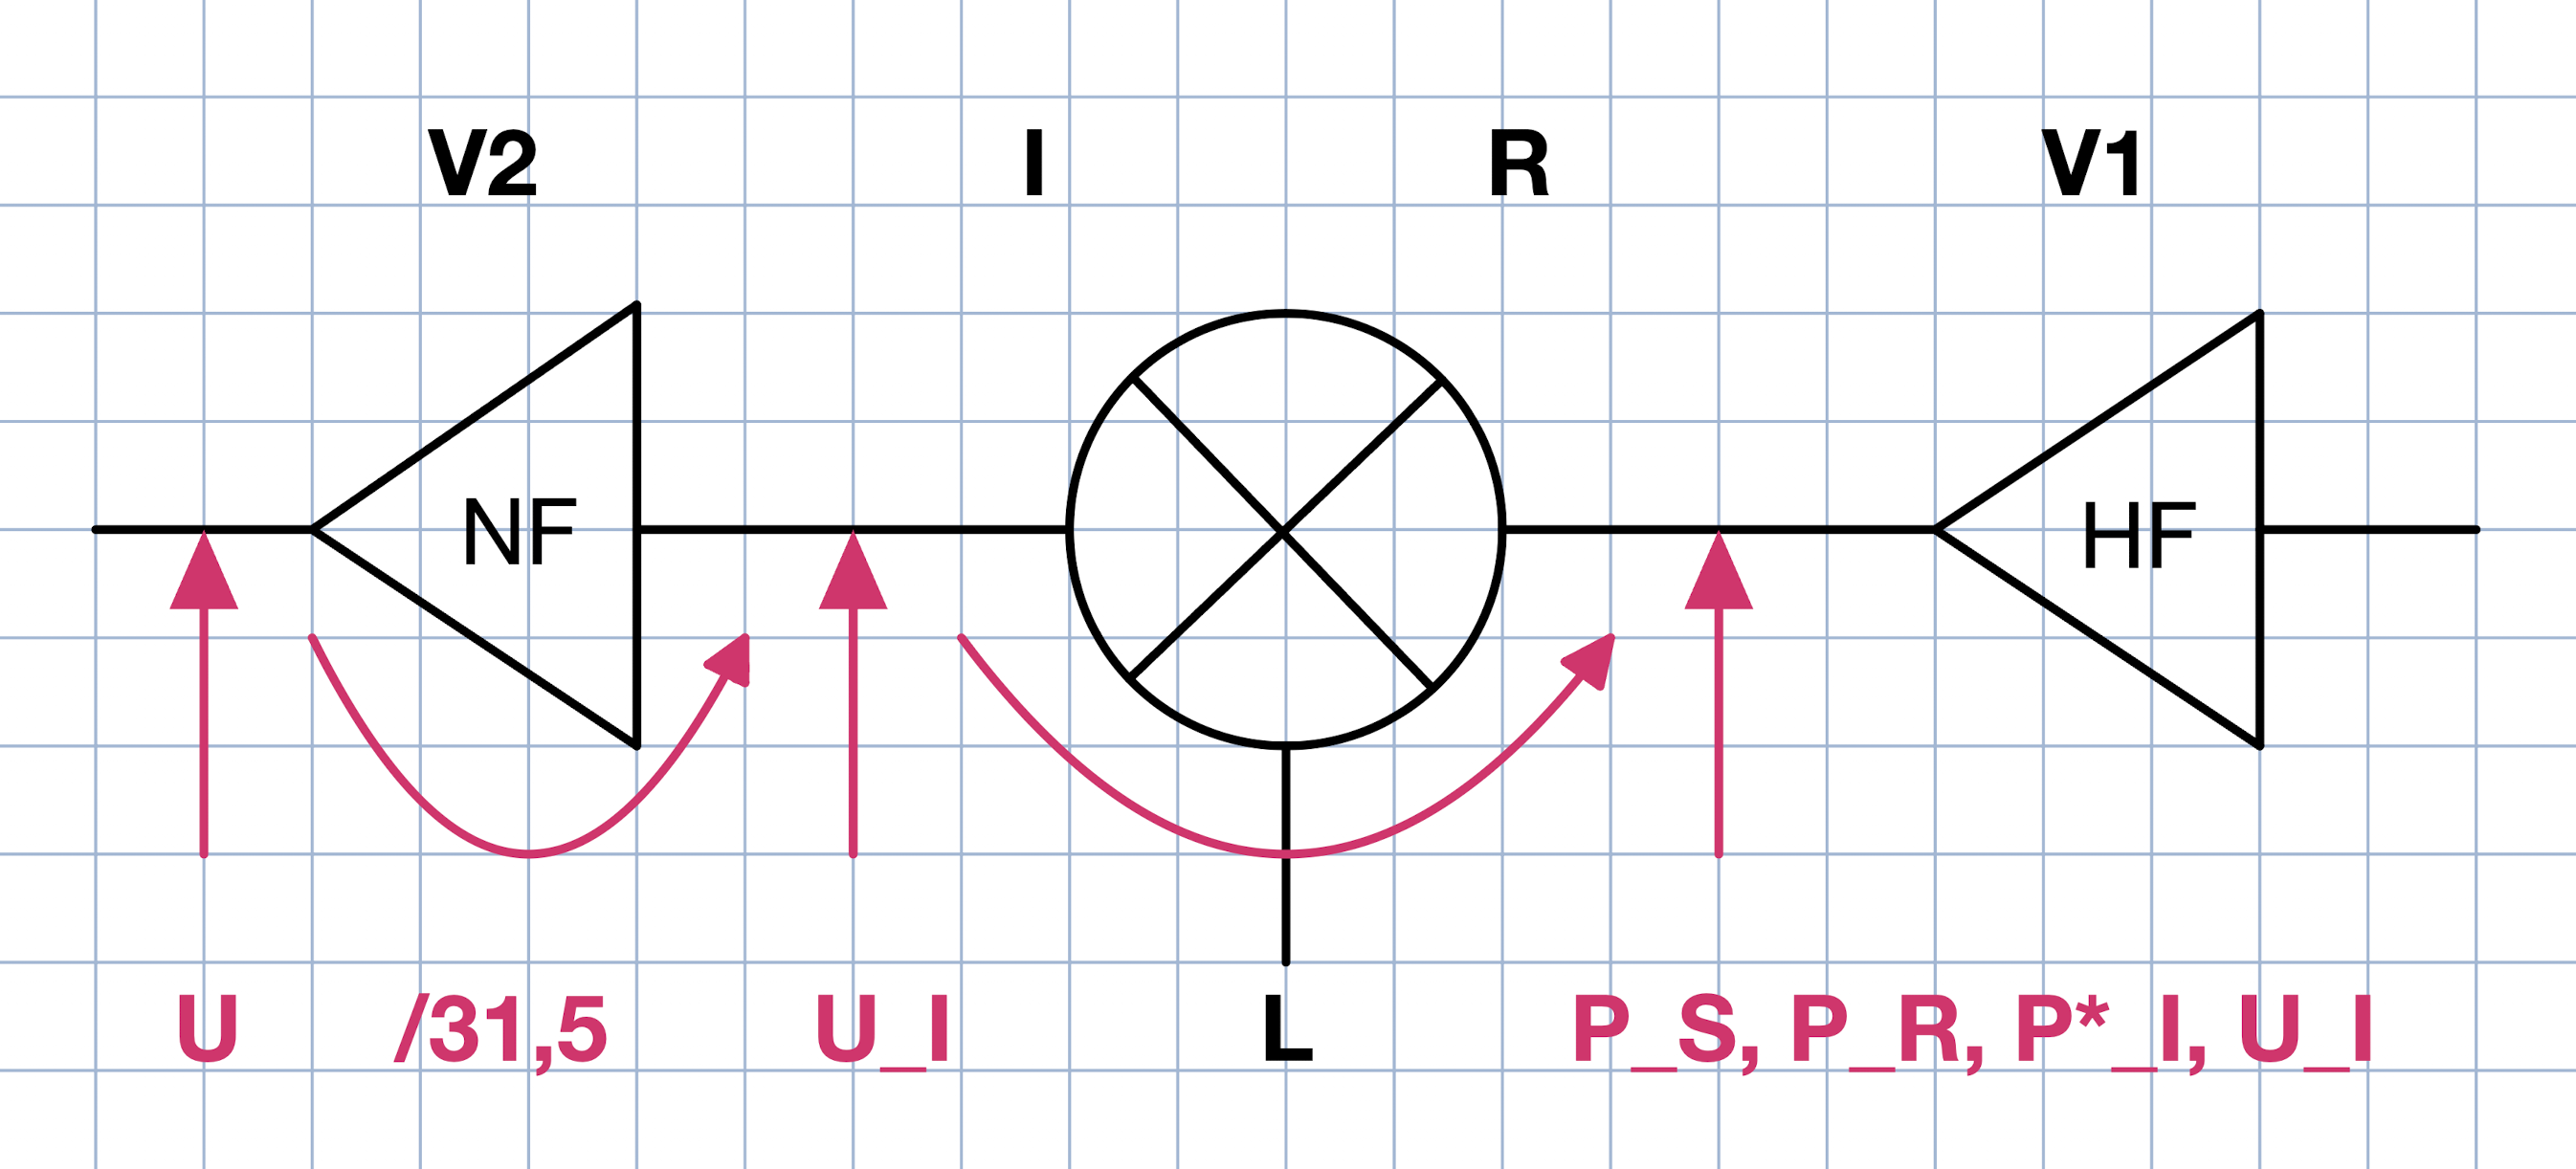
\includegraphics[scale=0.18]{Bilder/Schaltschema.png}
    \captionof{figure}{Skizze von der Anordnung der elektronischen Bauteile und Größen}
    \label{fig:schaltschema}
\end{center}

Die Spannung $U_\mathrm{I}$ wird dann durch die Formel:
\begin{gather}
    P^*_\mathrm{I} = 10\cdot\log_{10}\left(\frac{U_\mathrm{I}^2}{2R}\right);~~[P^*] = 1\,\mathrm{dBm}
\end{gather}
in den gesuchten HF-Leistungswerte ohne Mischer $P_\mathrm{I}^*$ umgerechnet. \cite{anleitung} Beachte hierbei, dass der Widerstand $R=50\,\Omega$ ist und dass auf $P_\mathrm{I}^*$ 6\,dBm dazuaddiert wurde, um den Vergleich zwischen $P_\mathrm{S,Mess}^*$ zu gewährleisten. \cite{anleitung} Alle berechneten Werte kann man in Tabelle \ref{tab:konversionsverluste} finden. Der Vergleich zwischen $P^*_\mathrm{I}$ und $P^*_\mathrm{S,Mess}$ wurde grafisch in Abb. \ref{fig:specAnalVergleich} dargestellt, wobei der Fehler weggelassen wurde da dieser zu klein zum Auflösen ist. 

Mittelung über die Ergebnisse ergibt dann:
\begin{gather}
    \boxed{\bar{P}_\mathrm{I}^* = (- 21,3 \pm 0,2)\,\mathrm{dBm}}~.
\end{gather}

Um dann die konkreten Konversionsverluste zu ermitteln wird der Abstand zwischen $\bar{P}^*_\mathrm{I}$ und $\bar{P}^*_\mathrm{S,Mess}$ HF-Leistungswerte berechnet und der Mittelwert gebildet sowie die Standardabweichung. Dafür wird die Größe $v = |\bar{P}^*_\mathrm{I} - \bar{P}^*_\mathrm{S,Mess}|$ als Konversionsverlust eingeführt. Die Berechnungen ergeben folgendes Ergebnis für den Konversionsverlust $v$:
\begin{gather}
    \boxed{v = (2 \pm 1)\,\mathrm{dBm}}~.
\end{gather}

\begin{center}
    \captionsetup{type=figure}
    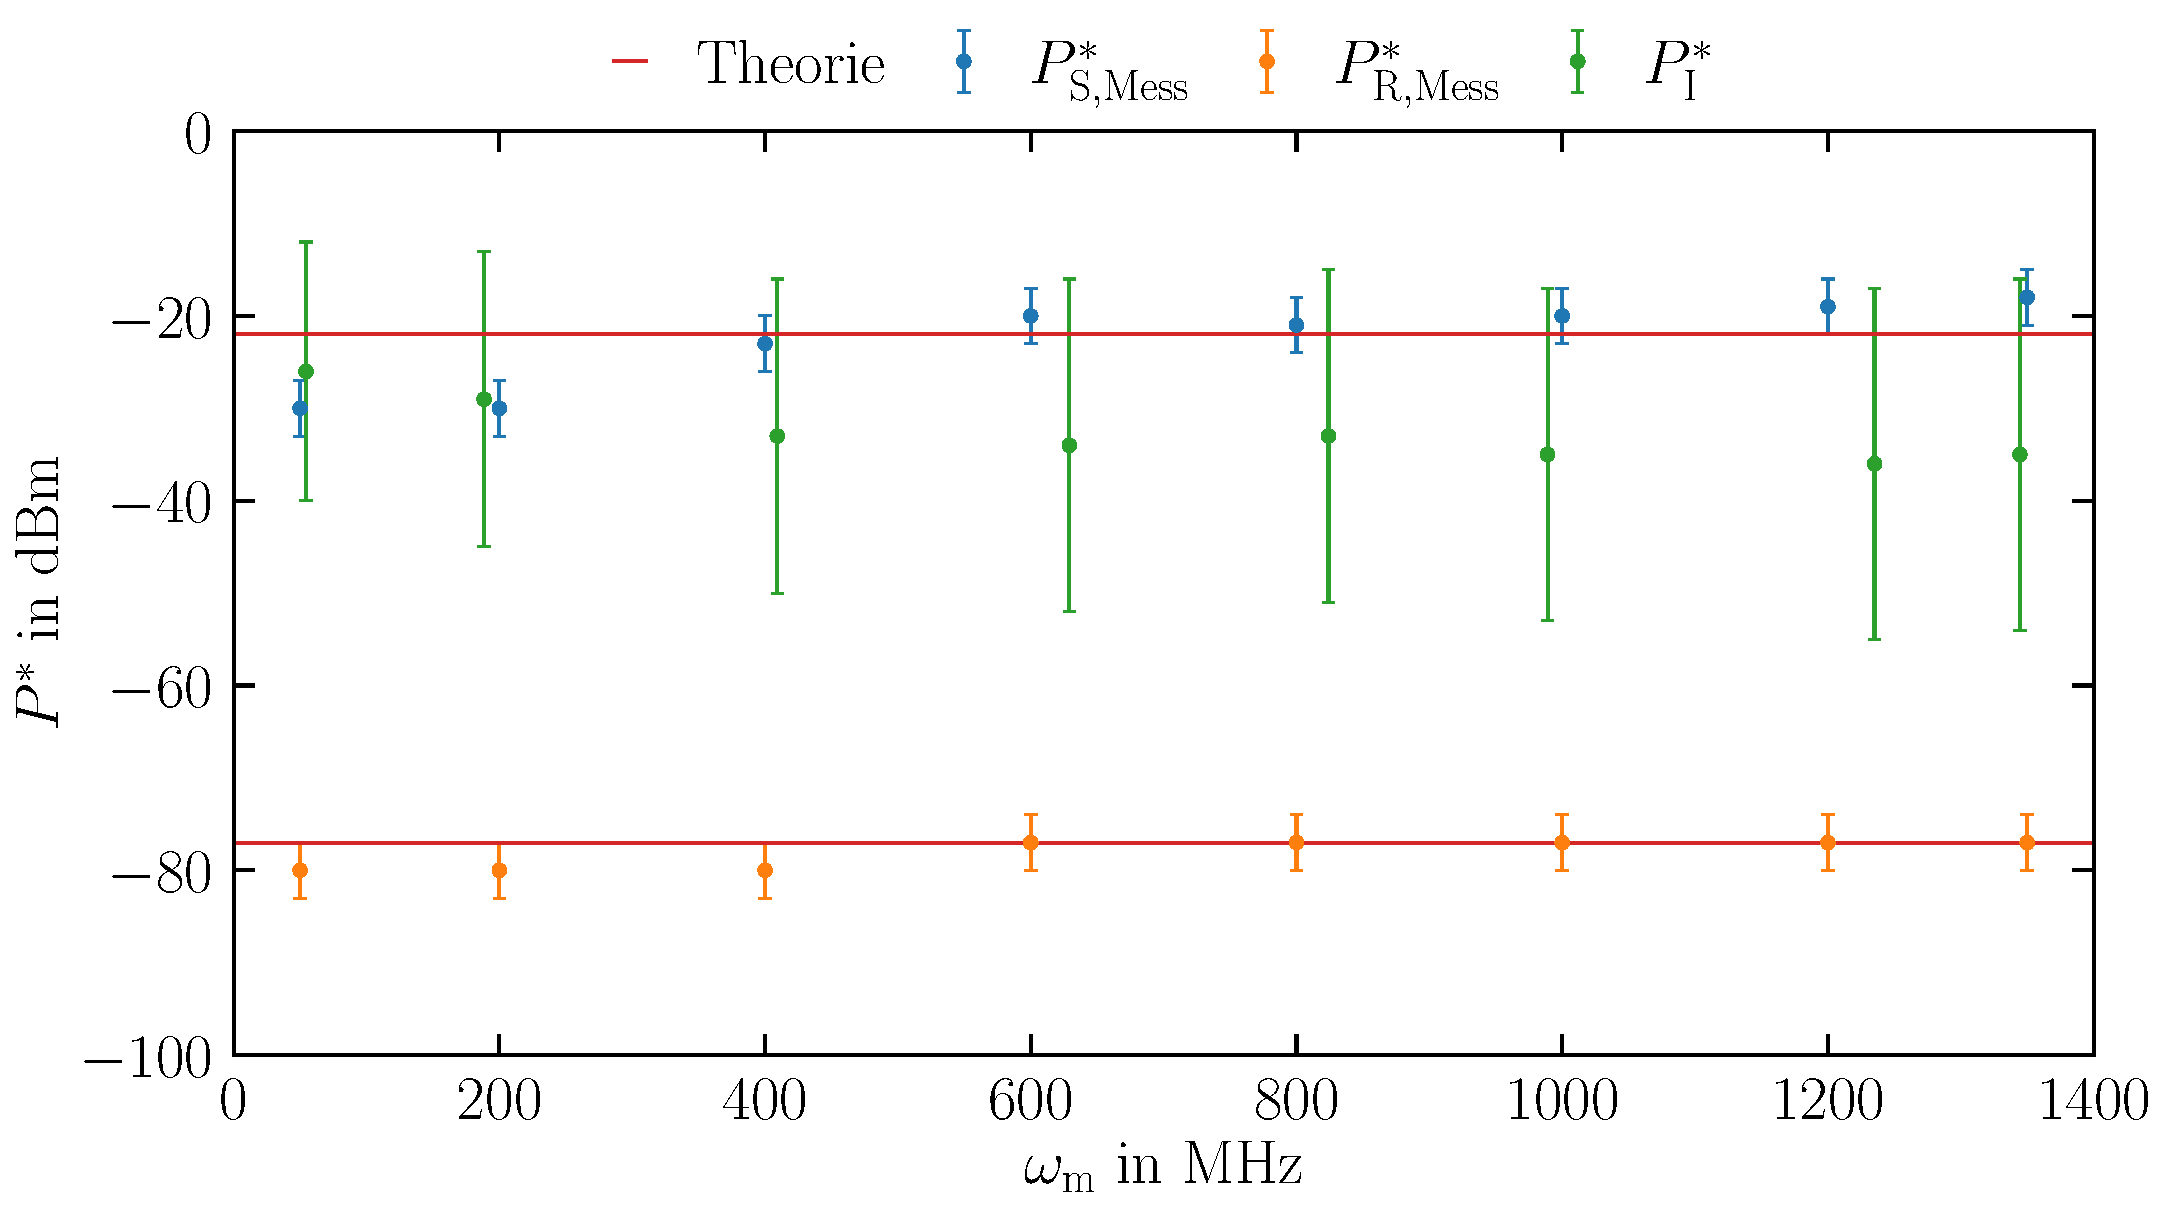
\includegraphics[scale=0.4]{Bilder/Auswertung/62/Signal-Rausch.pdf}
    \captionof{figure}{Vergleich zwischen Theorie und Praxis für gemessene Werte am Spektrumanalysator mit dem theoretischen Leistungswert des Rauschens \\$P^*_\mathrm{R,Theo}$ = -79\,dBm und des Signals $P^*_\mathrm{S,Theo}$= -30\,dBm, sowie gemessene Leistung mit Mischer $P^*_\mathrm{S,Mess}$ und ohne Mischer $P^* _\mathrm{I}$}
    \label{fig:specAnalVergleich}
\end{center}

\begin{center}
    \captionsetup{type=table}
    \begin{tabular}{r | c r | c c }
        $\omega_\mathrm{m}$/MHz & $U$/mV & $U_\mathrm{I}$/mV & $P_\mathrm{I}$/$10^{-4}$\,mW & $P^*_\mathrm{I}$/dBm \\ \hline
        54,5   & 208 $\pm$ 5 & 6,6  $\pm$ 0,2 & ~4,4 $\pm$ 0,3 & -27,6 $\pm$ 1,9 \\
        188,5  & 293 $\pm$ 5 & 9,3  $\pm$ 0,2 & ~8,6 $\pm$ 0,4 & -24,6 $\pm$ 1,1 \\
        409,2  & 421 $\pm$ 5 & 13,4 $\pm$ 0,2 & 18,0 $\pm$ 0,5 & -21,5 $\pm$ 0,6 \\
        629,1  & 511 $\pm$ 5 & 16,2 $\pm$ 0,2 & 26,2 $\pm$ 0,6 & -19,8 $\pm$ 0,5 \\
        824,1  & 452 $\pm$ 5 & 14,3 $\pm$ 0,2 & 20,4 $\pm$ 0,6 & -20,9 $\pm$ 0,6 \\
        989,0  & 533 $\pm$ 5 & 16,9 $\pm$ 0,2 & 28,6 $\pm$ 0,7 & -19,4 $\pm$ 0,5 \\
        1235,1 & 635 $\pm$ 5 & 20,2 $\pm$ 0,2 & 40,8 $\pm$ 0,8 & -17,9 $\pm$ 0,4 \\
        1344,5 & 572 $\pm$ 5 & 18,2 $\pm$ 0,2 & 33,1 $\pm$ 0,7 & -18,8 $\pm$ 0,4 \\
    \end{tabular}
    \captionof{table}{Berechnete Werte für Konversionsverluste mit der gemessenen Spanung $U$, der Spannung $U_\mathrm{I}$ am Ausgang I und die dazugehörge Leistung $P_\mathrm{I}$ in mW und dBm}
    \label{tab:konversionsverluste}
\end{center}

\subsection{Effektive Quantenausbeute}
\label{sub:ausbeute}

Im nächsten Abschnitt wird die Quantenausbeute $\beta_\mathrm{D}$ berechnet. Dafür wird Gleichung (\ref{eq:leistungPhotosignal}) aus Kapitel \ref{sec:signalRausch} verwendet und auf die Quantenausbeute $\beta_\mathrm{D}$ umgestellt:
\begin{gather}
    P_\mathrm{S} = \frac{R}{2}\left(\frac{e\beta_\mathrm{D}}{2hc}\lambda P M \frac{\ln10}{2}\mathrm{OD}\right)^2
    \quad \Leftrightarrow \quad \beta_\mathrm{D} = \underbrace{\sqrt{\frac{1}{\frac{R}{2}\left(\frac{e\beta_\mathrm{D}}{2hc}\lambda P\frac{\ln10}{2}\right)^2}}}_{C} \cdot \frac{\sqrt{P_\mathrm{S}}}{\mathrm{OD}\cdot M}~.
\end{gather}
Als Leistungswerte $P_\mathrm{S}$ werden die gemessenen Werte $P^*_\mathrm{S,Mess}$ aus Kapitel \ref{sub:specAnal} verwendet. Die optische Dichte OD ist in Kapitel \ref{sub:opDichte} als OD = 0,09 $\pm$ 0,07 gegeben. Weiterhin ist der Modulationsindex $M$ zu jeder Modulationsfrequenz $\omega_\mathrm{m}$ in Kapitel \ref{sec:mindex} zu finden. Für die Konstante $C$ gilt mit den Werten aus dem Skript \cite{anleitung} (auch in Kapitel \ref{sec:signalAbsorp} gegeben):
\begin{gather}
    C= 6807\,\sqrt{\mathrm{W}}~.
\end{gather}
Als Nächstes müssen die Leistungswerte $P^*_\mathrm{S,Mess}$ in mW umgerechnet werden, dafür wird der Verstärkungsfaktor von 55\,dB von $P^*_\mathrm{S,Mess}$ subtrahiert und dann mit der Formel:
\begin{gather}
    P^* = 10\log_{10}(P) \qquad \Leftrightarrow \qquad P = 10^{P^*/10}
    \label{eq:dBmTomW}
\end{gather}
umgerechnet. \cite{anleitung} Dabei ist $P^*$ der Leistungspegel in dBm und $P$ der Leistungspegel in mW. 
Tabelle \ref{tab:ausbeute} fasst nochmal alle Werte an einer Stelle zusammen, sowie die errechneten Werte für die Quantenausbeute $\beta_\mathrm{D}$. Messfehler wurden mit dem Fehlerfortpflanzungsgesetz berechnet. In Tabelle \ref{tab:ausbeute} lässt sich bei hohe Modulationsfrequenzen eine hohe Quantenausbeute $\beta_\mathrm{D}$ erkennen, aber auch einen sehr großen Messfehler aufgrund der deutlich höheren Leistungswerte. Dennoch lässt sich sagen, dass für niedrige Modulationsfrequenzen $\omega_\mathrm{m}$ die Quantenausbeute mit den Erwartungen on 0,3 \cite{anleitung} übereinstimmt. Betrachtet man den Mittelwert der Quantenausbeute $\beta_\mathrm{D}$ erhält man als Ergebnis:
\begin{gather}
    \boxed{\beta_\mathrm{D} = 0,73 \pm 0,22}~.
\end{gather}
Das Ergebnis liegt ein Stück über den Erwartungen, was aber auch mit dem systematischen Messfehler für Modulationsfrequenzen von 400 $\sim$ 1350\,MHz zu tun haben könnte.
Eine herkömmliche Silizium-Photodiode erreicht heutzutage eine Quantenausbeute von 80\,\%, wobei schon mit sogenannten schwarzen Silizium eine Quantenausbeute von 130\,\% gelungen ist. \cite{siPD} Dies lässt darauf schließen, dass die gemessenen Werte noch in der Erwartung der Realität liegen.
\begin{center}
    \captionsetup{type=table}
    \begin{tabular}{r | c c | c c}
        $\omega_\mathrm{m}$/MHz & $P^*_\mathrm{S,Mess}$/dBm & $P_\mathrm{S,Mess}$/$10^{-9}$\,mW & $M$ & $\beta_\mathrm{D}$\\ \hline
        50   & -85 $\pm$ 3 & ~3,16 $\pm$ 0.11 & 0,46 $\pm$ 0,03 & 0.29 $\pm$ 0.23 \\
        200  & -85 $\pm$ 3 & ~3,16 $\pm$ 0.11 & 0,52 $\pm$ 0,02 & 0.26 $\pm$ 0.20 \\
        400  & -78 $\pm$ 3 & 15,85 $\pm$ 0.61 & 0,50 $\pm$ 0,02 & 0.60 $\pm$ 0.47 \\
        600  & -75 $\pm$ 3 & 31,62 $\pm$ 1.26 & 0,54 $\pm$ 0,02 & 0.79 $\pm$ 0.62 \\
        800  & -76 $\pm$ 3 & 25,12 $\pm$ 0.99 & 0,46 $\pm$ 0,03 & 0.82 $\pm$ 0.64 \\
        1000 & -75 $\pm$ 3 & 31,62 $\pm$ 1.26 & 0,56 $\pm$ 0,02 & 0.76 $\pm$ 0.59 \\
        1200 & -74 $\pm$ 3 & 39,81 $\pm$ 1.61 & 0,46 $\pm$ 0,03 & 1.04 $\pm$ 0.81 \\
        1350 & -73 $\pm$ 3 & 50,12 $\pm$ 2.06 & 0,42 $\pm$ 0,03 & 1.27 $\pm$ 0.99 \\
    \end{tabular}
    \captionof{table}{Berechnete Werte für Quantenausbeute $\beta_\mathrm{D}$ mit den Leistungsweren des Signals $P_\mathrm{S}$ und den Modulatuionsindex $M$}
    \label{tab:ausbeute}
\end{center}

\subsection{Minimale optische Dichte}
\label{sub:minopDichte}

Um die minimale optische Dichte $\mathrm{OD}_\mathrm{min}$ der Messaperatur zu erhalten wird die Gleichung des thermischen Rauschens $P_\mathrm{T}$ mit der Gleichung (\ref{eq:leistungPhotosignal}) für die Lichtleistung $P_\mathrm{S}$ gleichgesetzt, dabei ist OD dann die minimale optische Dichte $\mathrm{OD}_\mathrm{min}$. Diese Überlegung hat dann das folgende Ergebnis zur Folge:
\begin{gather}
    P_\mathrm{T} = 4 k_\mathrm{B} T \Delta \nu = \frac{R}{2}\left(\frac{e\beta_\mathrm{D}}{2hc}\lambda P M \frac{\ln10}{2}\right)^2 \mathrm{OD}_\mathrm{min}  = P_\mathrm{S}~.
    \label{eq:signaleqrausch}
\end{gather}
Wenn man sich in Gleichung (\ref{eq:signaleqrausch}) den Term vor der minimalen optischen Dichte $\mathrm{OD}_\mathrm{min}$ genauer betrachtet, erkennt man, dass dieser Term wiederum in Gleichung (\ref{eq:leistungPhotosignal}) und das Verhältnis zwischen Lichtleistung $P_\mathrm{S}$ und optischer Dichte im Quadrat darstellt, also $P_\mathrm{S}/\mathrm{OD}^2$. Setzt man dies nun in Gleichung (\ref{eq:signaleqrausch}) ein und formt auf $\mathrm{OD}_\mathrm{min}$ um, erhält man:
\begin{gather}
    \Rightarrow \qquad \boxed{\mathrm{OD}_\mathrm{min} = \sqrt{\frac{P_\mathrm{T}}{P_\mathrm{S}}} \cdot \mathrm{OD}}~,
    \label{eq:minopDichte}
\end{gather}
wobei $\mathrm{OD}$ die gemessene optische Dichte mit $0,09 \pm 0,07$ aus Kapitel \ref{sub:opDichte} ist. Als Leistungswerte $P_\mathrm{T}$ und $P_\mathrm{S}$ werden die berechneten Werte aus Kapitel \ref{sec:rauschen} ($P_\mathrm{R,Theo}$) und \ref{sec:signalAbsorp} ($P_\mathrm{S,Theo}$)  verwendet. Dabei wird aber der Wert von $P_\mathrm{R,Theo}$ durch 4 gerechnet \cite{anleitung}, da die Formel für $P_\mathrm{S,Theo}$ schon für die gemessenen Werte angepasst wurde. Die Fehler wurde wieder mit dem Fehlerfortpflanzungsgesetz ermittelt und damit folgt für die minimale optische Dichte:
\begin{gather}
    \boxed{\mathrm{OD}_\mathrm{min} = (3,25 \pm 2,53) \cdot 10^{-4}}~.
\end{gather}

%\begin{center}
%    \captionsetup{type=table}
%    \begin{tabular}{r | c c c | c}
%        $\omega_\mathrm{m}$/MHz & $P^*_\mathrm{S,Mess}$/dBm & $P^*_\mathrm{R,Mess}$/mW & $\Delta P^*$/dBm & $ \mathrm{OD}_\mathrm{min} \cdot 10^{-6}$ \\ \hline
%        50   & -30 $\pm$ 3 & -80 $\pm$ 3 & -50 $\pm$ 4 & 0.90 $\pm$ 1.08 \\
%        200  & -30 $\pm$ 3 & -80 $\pm$ 3 & -50 $\pm$ 4 & 0.90 $\pm$ 1.08 \\
%        400  & -23 $\pm$ 3 & -80 $\pm$ 3 & -57 $\pm$ 4 & 0.18 $\pm$ 0.22 \\
%        600  & -20 $\pm$ 3 & -77 $\pm$ 3 & -57 $\pm$ 4 & 0.18 $\pm$ 0.22 \\
%        800  & -21 $\pm$ 3 & -77 $\pm$ 3 & -56 $\pm$ 4 & 0.23 $\pm$ 0.27 \\
%        1000 & -20 $\pm$ 3 & -77 $\pm$ 3 & -57 $\pm$ 4 & 0.18 $\pm$ 0.22 \\
%        1200 & -19 $\pm$ 3 & -77 $\pm$ 3 & -58 $\pm$ 4 & 0.14 $\pm$ 0.17 \\
%        1350 & -18 $\pm$ 3 & -77 $\pm$ 3 & -59 $\pm$ 4 & 0.11 $\pm$ 0.14 \\
%    \end{tabular}
%    \captionof{table}{Berechnete Werte für minimale optische Dichte}
%    \label{tab:minopDichte}
%\end{center}








